\documentclass[12pt]{article}

\title{Initial conditions}
\author{Jan Medlock et al.}

\usepackage{microtype}
\usepackage{tikz}
\usepackage{hyperref}
\hypersetup{breaklinks}
\hypersetup{pdfborder=0 0 0}
\usepackage{natbib}
\usepackage{hypernat}
\usepackage{amsmath}
\renewcommand{\vec}[1]{\mathbf{#1}}
\newcommand{\mat}[1]{\mathbf{#1}}
\DeclareMathOperator{\Prob}{Prob}
\DeclareMathOperator{\diag}{diag}
\newcommand{\md}{\mathrm{d}}
\newcommand{\me}{\mathrm{e}}
\newcommand{\mT}{\mathrm{T}}
\setcounter{MaxMatrixCols}{12}


\begin{document}

\maketitle

We will find the equilibrium probability as a function of age of being
in each model compartment (\autoref{model_diagram}), i.e.
\begin{equation}
  P_X(a) = \Prob\{\text{in compartment $X$ at age $a$}|\text{alive at
    age $a$}\},
\end{equation}
for $X \in \{\mathrm{M}, \mathrm{S}, \mathrm{E}, \mathrm{I}, \mathrm{R}\}$
and $a \geq 0$.
We will assume that
\begin{itemize}
\item the infection hazard is constant, and
\item all calves are born with maternal immunity.
\end{itemize}

\begin{figure}
  \begin{center}
    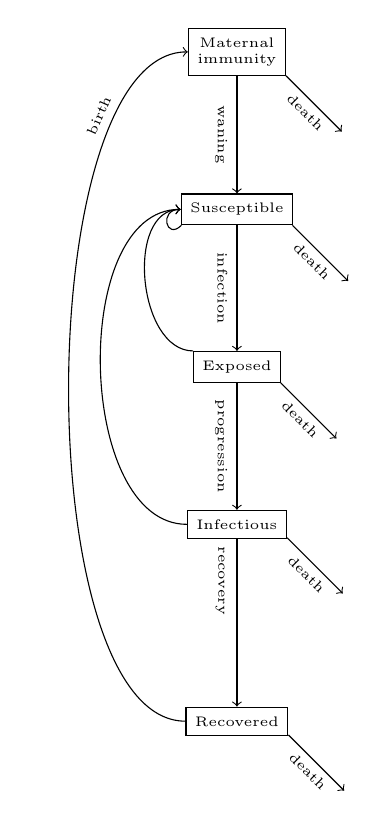
\begin{tikzpicture}[compartment/.style = {rectangle, draw}, font=\fontsize{5pt}{6}\selectfont]
  % Compartments.
  \node at (0, 11) [compartment, align=center, name=MaternalImmunity] {Maternal\\immunity};
  \node at (0, 9) [compartment, name=Susceptible] {Susceptible};
  \node at (0, 7) [compartment, name=Exposed] {Exposed};
  \node at (0, 5) [compartment, name=Infectious] {Infectious};
  \node at (0, 2.5) [compartment, name=Recovered] {Recovered};

  % Location for branch from Infectious to Chronic and Recovered.
  \coordinate (recovery) at (0, 3.75);

  % Infection-related processes.
  \draw [->] (MaternalImmunity)
             to node [rotate=-90, below] {waning}
             (Susceptible);
  \draw [->] (Susceptible)
             to node [rotate=-90, below] {infection}
             (Exposed);
  \draw [->] (Exposed)
             to node [rotate=-90, below] {progression}
             (Infectious);
  \draw [  ] (Infectious)
             to node [rotate=-90, below, yshift=-1pt] {recovery}
             (recovery);
  \draw [->] (recovery)
             to node [] {}
             (Recovered.90);

  % Births
  \draw [->] (Susceptible.196)
             to [out=225, in=180, looseness=3.5] node [] {}
             (Susceptible.180);
  \draw [->] (Exposed.160)
             to [out=180, in=180] node [] {}
             (Susceptible.180);
  \draw [->] (Infectious.180)
             to [out=180, in=180, looseness=0.9] node [sloped, above, pos=0.85] {}
             (Susceptible.180);
  \draw [->] (Recovered.180)
             to [out=180, in=180, looseness=0.6] node [sloped, above, pos=0.8] {birth}
             (MaternalImmunity.180);

  % Deaths
  \draw [->] (MaternalImmunity.334)
             to node [sloped, below, yshift=1pt] {death}
             +(315: 1);
  \draw [->] (Susceptible.344)
             to node [sloped, below, yshift=1pt] {death}
             +(315: 1);
  \draw [->] (Exposed.340)
             to node [sloped, below, yshift=1pt] {death}
             +(315: 1);
  \draw [->] (Infectious.345)
             to node [sloped, below, yshift=1pt] {death}
             +(315: 1);
  \draw [->] (Recovered.345)
             to node [sloped, below, yshift=1pt] {death}
             +(315: 1);
\end{tikzpicture}

%%% Local Variables:
%%% mode: latex
%%% TeX-master: "diagram_standalone"
%%% End:

  \end{center}
  \caption{Model diagram.}
  \label{model_diagram}
\end{figure}

\clearpage

For $a > 0$ and $0 < r < a$,
the compartment probabilities satisfy
\begin{align}
  P_{\mathrm{M}}(0) &= 1,
  \\
  \frac{\md P_{\mathrm{M}}}{\md a}
  &= - h_{\text{waning}}(a) P_{\mathrm{M}}(a),
  \displaybreak[0]\\
  P_{\mathrm{S}}(0) &= 0,
  \\
  \frac{\md P_{\mathrm{S}}}{\md a}
  &= h_{\text{waning}}(a) P_{\mathrm{M}}(a)
  - h_{\text{infection}} P_{\mathrm{S}}(a),
  \displaybreak[0]\\
  p_{\mathrm{E}}(0, 0) &= 0,
  \\
  p_{\mathrm{E}}(a, 0) &= h_{\text{infection}} P_{\mathrm{S}}(a),
  \\
  \frac{\partial p_{\mathrm{E}}}{\partial a}
  + \frac{\partial p_{\mathrm{E}}}{\partial r}
  &= - h_{\text{progression}}(r) p_{\mathrm{E}}(a, r),
  \displaybreak[0]\\
  p_{\mathrm{I}}(0, 0) &= 0,
  \\
  p_{\mathrm{I}}(a, 0) &=
  \int_0^a h_{\text{progression}}(r)
  p_{\mathrm{E}}(a, r) \md r,
  \\
  \frac{\partial p_{\mathrm{I}}}{\partial a}
  + \frac{\partial p_{\mathrm{I}}}{\partial r}
  &= - h_{\text{recovery}}(r) p_{\mathrm{I}}(a, r),
  \\
  P_{\mathrm{R}}(0) &= 0,
  \\
  \frac{\md P_{\mathrm{R}}}{\md a} &=
  \int_0^a h_{\text{recovery}}(r) p_{\mathrm{I}}(a, r) \md r,
\end{align}
with
\begin{align}
  P_{\mathrm{E}}(a) &= \int_0^a p_{\mathrm{E}}(a, r) \md r,
  \\
  P_{\mathrm{I}}(a) &= \int_0^a p_{\mathrm{I}}(a, r) \md r.
\end{align}

Let
\begin{equation}
  P(a) = P_{\mathrm{M}}(a) + P_{\mathrm{S}}(a)
  + P_{\mathrm{E}}(a) + P_{\mathrm{I}}(a)
  + P_{\mathrm{R}}(a),
\end{equation}
so that
\begin{equation}
  \begin{split}
    \frac{\md P_{\mathrm{E}}}{\md a}
    &= \frac{\md}{\md a}  \int_0^a p_{\mathrm{E}}(a, r) \md r
    \\
    &= p_{\mathrm{E}}(a, a)
    + \int_0^a \frac{\partial p_{\mathrm{E}}}{\partial a} \md r
    \\
    &= p_{\mathrm{E}}(a, a)
    - \int_0^a \frac{\partial p_{\mathrm{E}}}{\partial r}
    + h_{\mathrm{progression}}(r) p_{\mathrm{E}}(a, r) \md r
    \\
    &= p_{\mathrm{E}}(a, 0)
    - \int_0^a h_{\mathrm{progression}}(r) p_{\mathrm{E}}(a, r) \md r,
    \\
    &= h_{\mathrm{infection}} P_{\mathrm{S}}(a)
    - \int_0^a h_{\mathrm{progression}}(r) p_{\mathrm{E}}(a, r) \md r,
  \end{split}
\end{equation}
\begin{equation}
  \begin{split}
    \frac{\md P_{\mathrm{I}}}{\md a}
    &= \frac{\md}{\md a}  \int_0^a p_{\mathrm{I}}(a, r) \md r
    \\
    &= p_{\mathrm{I}}(a, a)
    + \int_0^a \frac{\partial p_{\mathrm{I}}}{\partial a} \md r
    \\
    &= p_{\mathrm{I}}(a, a)
    - \int_0^a \frac{\partial p_{\mathrm{I}}}{\partial r} \md r
    \\
    &= p_{\mathrm{I}}(a, 0)
    \\
    &= \int_0^a h_{\mathrm{progression}}(r) p_{\mathrm{E}}(a, r) \md r,
  \end{split}
\end{equation}
and then
\begin{equation}
  \frac{\md P}{\md a} =
  \frac{\md P_{\mathrm{M}}}{\md a}
  + \frac{\md P_{\mathrm{S}}}{\md a}
  + \frac{\md P_{\mathrm{E}}}{\md a}
  + \frac{\md P_{\mathrm{I}}}{\md a}
  + \frac{\md P_{\mathrm{R}}}{\md a}
  = 0.
\end{equation}


\section{Numerical method}

To compute the compartment probabilities, we used the Crank--Nicolson
method on characteristics and the composite trapezoid rule for the
integrals \citep{milner_1992}.  Given the age step $\Delta a$,
for $i \in \{0, 1, 2, \ldots, I - 1\}$ and $j \in \{0, 1, 2,
\ldots, i - 1\}$, let $a^i = i \Delta a$, $r^j = j \Delta a$,
$P_X^i \approx P_X(a^i)$, and $p_X^{i, j} \approx
p_X(a^i, r^j)$.
For each $1 \leq i \leq I - 1$ and each $1 \leq j \leq i - 1$, the
Crank--Nicolson method on characteristics is
\begin{align}
  P_{\mathrm{M}}^0 &= 1,
  \\
  \frac{P_{\mathrm{M}}^i - P_{\mathrm{M}}^{i - 1}}{\Delta a}
  &= - h_{\text{waning}}(a^{i - 1 / 2})
  \frac{P_{\mathrm{M}}^i + P_{\mathrm{M}}^{i - 1}}{2},
  \displaybreak[0]\\
  P_{\mathrm{S}}^0 &= 0,
  \\
  \frac{P_{\mathrm{S}}^i - P_{\mathrm{S}}^{i - 1}}{\Delta a}
  &= h_{\text{waning}}(a^{i - 1 / 2})
  \frac{P_{\mathrm{M}}^i + P_{\mathrm{M}}^{i - 1}}{2}
  - h_{\text{infection}}
  \frac{P_{\mathrm{S}}^i + P_{\mathrm{S}}^{i - 1}}{2},
  \displaybreak[0]\\
  p_{\mathrm{E}}^{i, 0} &= h_{\text{infection}}
  \frac{P_{\mathrm{S}}^i + P_{\mathrm{S}}^{i - 1}}{2},
  \\
  \frac{p_{\mathrm{E}}^{i, j} - p_{\mathrm{E}}^{i - 1, j - 1}}{\Delta a}
  &= - h_{\text{progression}}(r^{j - 1 / 2})
  \frac{p_{\mathrm{E}}^{i, j} + p_{\mathrm{E}}^{i - 1, j - 1}}{2},
  \displaybreak[0]\\
  p_{\mathrm{I}}^{i, 0} &=
  \sum_{j = 1}^{i - 1} h_{\text{progression}}(r^{j - 1 / 2})
  \frac{p_{\mathrm{E}}^{i, j} + p_{\mathrm{E}}^{i - 1, j - 1}}{2}
  \Delta a,
  \\
  \frac{p_{\mathrm{I}}^{i, j} - p_{\mathrm{I}}^{i - 1, j - 1}}{\Delta a}
  &= - h_{\text{recovery}}(r^{j - 1 / 2})
  \frac{p_{\mathrm{I}}^{i, j} + p_{\mathrm{I}}^{i - 1, j - 1}}{2},
  \displaybreak[0]\\
  P_{\mathrm{R}}^0 &= 0,
  \\
  \frac{P_{\mathrm{R}}^i - P_{\mathrm{R}}^{i - 1}}{\Delta a}
  &= \sum_{j = 1}^{i - 1} h_{\text{recovery}}(r^{j - 1 / 2})
  \frac{p_{\mathrm{I}}^{i, j} + p_{\mathrm{I}}^{i - 1, j - 1}}{2}
  \Delta a,
\end{align}
Then
\begin{align}
  P_{\mathrm{E}}^0 &= 0,
  \\
  P_{\mathrm{E}}^i &= \sum_{j = 0}^{i - 1} p_{\mathrm{E}}^{i, j} \Delta a,
  \\
  P_{\mathrm{I}}^0 &= 0,
  \\
  P_{\mathrm{I}}^i &= \sum_{j = 0}^{i - 1} p_{\mathrm{I}}^{i, j} \Delta a.
\end{align}

For the variables $P_X$ that only depend on age $a$,
define the vectors
\begin{equation}
  \vec{P}_X =
  \begin{pmatrix}
    P_X^0\\
    P_X^1\\
    \vdots\\
    P_X^{I - 1}
  \end{pmatrix},
\end{equation}
for $X \in \{\mathrm{M}, \mathrm{S}, \mathrm{R}\}$.
For the variables that depend on age $a$ and residence time $r$,
define the vectors
\begin{equation}
  \vec{p}_X =
  \begin{pmatrix}
    p_X^{1, 0}\\
    p_X^{2, 0}\\
    p_X^{2, 1}\\
    p_X^{3, 0}\\
    p_X^{3, 1}\\
    p_X^{3, 2}\\
    \vdots\\
    p_X^{I - 1, 0}\\
    \vdots\\
    p_X^{I - 1, I - 2}
  \end{pmatrix},
\end{equation}
for $X \in \{\mathrm{E}, \mathrm{I}\}$,
where the $i, j$th entry is in position
\begin{equation}
  k = \frac{i (i - 1)}{2} + j,
\end{equation}
or
\begin{align}
  i &= \left\lfloor\frac{1 + \sqrt{8 k + 1}}{2}\right\rfloor,
  \\
  j &= k - \frac{i (i - 1)}{2}.
\end{align}
Then for $1 \leq i \leq I - 1$ and $1 \leq j \leq i - 1$,
\begin{align}
  P_{\mathrm{M}}^0 &= 1,
  \\
  - \frac{2 - h_{\text{waning}}(a^{i - 1 / 2}) \Delta a}
  {2 + h_{\text{waning}}(a^{i - 1 / 2}) \Delta a}
  P_{\mathrm{M}}^{i - 1}
  + P_{\mathrm{M}}^i
  &= 0,
  \displaybreak[0]\\
  P_{\mathrm{S}}^0 &= 0,
  \\
  \begin{split}
    - \frac{h_{\text{waning}}(a^{i - 1 / 2}) \Delta a}
    {2 + h_{\text{infection}} \Delta a}
    P_{\mathrm{M}}^{i - 1}
    - \frac{h_{\text{waning}}(a^{i - 1 / 2}) \Delta a}
    {2 + h_{\text{infection}} \Delta a}
    P_{\mathrm{M}}^i
    \\ {}
    - \frac{2 - h_{\text{infection}} \Delta a}
    {2 + h_{\text{infection}} \Delta a}
    P_{\mathrm{S}}^{i - 1}
    + P_{\mathrm{S}}^i
    &= 0,
  \end{split}
  \displaybreak[0]\\
  P_{\mathrm{R}}^0 &= 0,
  \\
  \begin{split}
    - \sum_{j = 1}^{i - 1}
    \frac{h_{\text{recovery}}(r^{j - 1 / 2}) (\Delta a)^2}{2}
    p_{\mathrm{I}}^{i - 1, j - 1}
    \\ {}
    - \sum_{j = 1}^{i - 1}
    \frac{h_{\text{recovery}}(r^{j - 1 / 2}) (\Delta a)^2}{2}
    p_{\mathrm{I}}^{i, j}
    \\ {}
    - P_{\mathrm{R}}^{i - 1} + P_{\mathrm{R}}^i
    &= 0,
  \end{split}
  \displaybreak[0]\\
  - \frac{h_{\text{infection}}}{2} P_{\mathrm{S}}^{i - 1}
  - \frac{h_{\text{infection}}}{2} P_{\mathrm{S}}^i
  + p_{\mathrm{E}}^{i, 0}
  &= 0,
  \\
  - \frac{2 - h_{\text{progression}}(r^{j - 1 / 2}) \Delta a}
  {2 + h_{\text{progression}}(r^{j - 1 / 2}) \Delta a}
  p_{\mathrm{E}}^{i - 1, j - 1}
  + p_{\mathrm{E}}^{i, j}
  &= 0,
  \displaybreak[0]\\
  \begin{split}
    - \sum_{j = 1}^{i - 1}
    \frac{h_{\text{progression}}(r^{j - 1 / 2}) \Delta a}{2}
    p_{\mathrm{E}}^{i - 1, j - 1}
    - \sum_{j = 1}^{i - 1}
    \frac{h_{\text{progression}}(r^{j - 1 / 2}) \Delta a}{2}
    p_{\mathrm{E}}^{i, j}
    \\ {}
    + p_{\mathrm{I}}^{i, 0}
    &= 0,
  \end{split}
  \\
  - \frac{2 - h_{\text{recovery}}(r^{j - 1 / 2}) \Delta a}
  {2 + h_{\text{recovery}}(r^{j - 1 / 2}) \Delta a}
  p_{\mathrm{I}}^{i - 1, j - 1}
  + p_{\mathrm{I}}^{i, j}
  &= 0.
\end{align}
The coefficients must be non-negative to ensure each component of the
$P_X$'s and $p_X$'s is non-negative. In particular, the hazards must
satisfy
\begin{equation}
  2 - h \Delta a \geq 0,
\end{equation}
or
\begin{equation}
  h \leq \frac{2}{\Delta a}.
\end{equation}


\bibliography{journal_abbreviations,math_epi}
\bibliographystyle{jpmbib}

\end{document}
